\documentclass[1p]{elsarticle_modified}
%\bibliographystyle{elsarticle-num}

%\usepackage[colorlinks]{hyperref}
%\usepackage{abbrmath_seonhwa} %\Abb, \Ascr, \Acal ,\Abf, \Afrak
\usepackage{amsfonts}
\usepackage{amssymb}
\usepackage{amsmath}
\usepackage{amsthm}
\usepackage{scalefnt}
\usepackage{amsbsy}
\usepackage{kotex}
\usepackage{caption}
\usepackage{subfig}
\usepackage{color}
\usepackage{graphicx}
\usepackage{xcolor} %% white, black, red, green, blue, cyan, magenta, yellow
\usepackage{float}
\usepackage{setspace}
\usepackage{hyperref}

\usepackage{tikz}
\usetikzlibrary{arrows}

\usepackage{multirow}
\usepackage{array} % fixed length table
\usepackage{hhline}

%%%%%%%%%%%%%%%%%%%%%
\makeatletter
\renewcommand*\env@matrix[1][\arraystretch]{%
	\edef\arraystretch{#1}%
	\hskip -\arraycolsep
	\let\@ifnextchar\new@ifnextchar
	\array{*\c@MaxMatrixCols c}}
\makeatother %https://tex.stackexchange.com/questions/14071/how-can-i-increase-the-line-spacing-in-a-matrix
%%%%%%%%%%%%%%%

\usepackage[normalem]{ulem}

\newcommand{\msout}[1]{\ifmmode\text{\sout{\ensuremath{#1}}}\else\sout{#1}\fi}
%SOURCE: \msout is \stkout macro in https://tex.stackexchange.com/questions/20609/strikeout-in-math-mode

\newcommand{\cancel}[1]{
	\ifmmode
	{\color{red}\msout{#1}}
	\else
	{\color{red}\sout{#1}}
	\fi
}

\newcommand{\add}[1]{
	{\color{blue}\uwave{#1}}
}

\newcommand{\replace}[2]{
	\ifmmode
	{\color{red}\msout{#1}}{\color{blue}\uwave{#2}}
	\else
	{\color{red}\sout{#1}}{\color{blue}\uwave{#2}}
	\fi
}

\newcommand{\Sol}{\mathcal{S}} %segment
\newcommand{\D}{D} %diagram
\newcommand{\A}{\mathcal{A}} %arc


%%%%%%%%%%%%%%%%%%%%%%%%%%%%%5 test

\def\sl{\operatorname{\textup{SL}}(2,\Cbb)}
\def\psl{\operatorname{\textup{PSL}}(2,\Cbb)}
\def\quan{\mkern 1mu \triangleright \mkern 1mu}

\theoremstyle{definition}
\newtheorem{thm}{Theorem}[section]
\newtheorem{prop}[thm]{Proposition}
\newtheorem{lem}[thm]{Lemma}
\newtheorem{ques}[thm]{Question}
\newtheorem{cor}[thm]{Corollary}
\newtheorem{defn}[thm]{Definition}
\newtheorem{exam}[thm]{Example}
\newtheorem{rmk}[thm]{Remark}
\newtheorem{alg}[thm]{Algorithm}

\newcommand{\I}{\sqrt{-1}}
\begin{document}

%\begin{frontmatter}
%
%\title{Boundary parabolic representations of knots up to 8 crossings}
%
%%% Group authors per affiliation:
%\author{Yunhi Cho} 
%\address{Department of Mathematics, University of Seoul, Seoul, Korea}
%\ead{yhcho@uos.ac.kr}
%
%
%\author{Seonhwa Kim} %\fnref{s_kim}}
%\address{Center for Geometry and Physics, Institute for Basic Science, Pohang, 37673, Korea}
%\ead{ryeona17@ibs.re.kr}
%
%\author{Hyuk Kim}
%\address{Department of Mathematical Sciences, Seoul National University, Seoul 08826, Korea}
%\ead{hyukkim@snu.ac.kr}
%
%\author{Seokbeom Yoon}
%\address{Department of Mathematical Sciences, Seoul National University, Seoul, 08826,  Korea}
%\ead{sbyoon15@snu.ac.kr}
%
%\begin{abstract}
%We find all boundary parabolic representation of knots up to 8 crossings.
%
%\end{abstract}
%\begin{keyword}
%    \MSC[2010] 57M25 
%\end{keyword}
%
%\end{frontmatter}

%\linenumbers
%\tableofcontents
%
\newcommand\colored[1]{\textcolor{white}{\rule[-0.35ex]{0.8em}{1.4ex}}\kern-0.8em\color{red} #1}%
%\newcommand\colored[1]{\textcolor{white}{ #1}\kern-2.17ex	\textcolor{white}{ #1}\kern-1.81ex	\textcolor{white}{ #1}\kern-2.15ex\color{red}#1	}

{\Large $\underline{11n_{113}~(K11n_{113})}$}

\setlength{\tabcolsep}{10pt}
\renewcommand{\arraystretch}{1.6}
\vspace{1cm}\begin{tabular}{m{100pt}>{\centering\arraybackslash}m{274pt}}
\multirow{5}{120pt}{
	\centering
	\includegraphics[width=112pt]{../../../GIT/diagram.site/Diagrams/png/729_11n_113.png}\\
\ \ \ A knot diagram\footnotemark}&
\allowdisplaybreaks
\textbf{Linearized knot diagam} \\
\cline{2-2}
 &
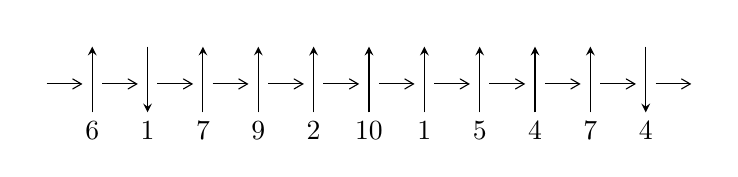
\begin{tikzpicture}[x=20pt, y=17pt]
	% nodes
	\node (C0) at (0, 0) {};
	\node (C1) at (1, 0) {};
	\node (C1U) at (1, +1) {};
	\node (C1D) at (1, -1) {6};

	\node (C2) at (2, 0) {};
	\node (C2U) at (2, +1) {};
	\node (C2D) at (2, -1) {1};

	\node (C3) at (3, 0) {};
	\node (C3U) at (3, +1) {};
	\node (C3D) at (3, -1) {7};

	\node (C4) at (4, 0) {};
	\node (C4U) at (4, +1) {};
	\node (C4D) at (4, -1) {9};

	\node (C5) at (5, 0) {};
	\node (C5U) at (5, +1) {};
	\node (C5D) at (5, -1) {2};

	\node (C6) at (6, 0) {};
	\node (C6U) at (6, +1) {};
	\node (C6D) at (6, -1) {10};

	\node (C7) at (7, 0) {};
	\node (C7U) at (7, +1) {};
	\node (C7D) at (7, -1) {1};

	\node (C8) at (8, 0) {};
	\node (C8U) at (8, +1) {};
	\node (C8D) at (8, -1) {5};

	\node (C9) at (9, 0) {};
	\node (C9U) at (9, +1) {};
	\node (C9D) at (9, -1) {4};

	\node (C10) at (10, 0) {};
	\node (C10U) at (10, +1) {};
	\node (C10D) at (10, -1) {7};

	\node (C11) at (11, 0) {};
	\node (C11U) at (11, +1) {};
	\node (C11D) at (11, -1) {4};
	\node (C12) at (12, 0) {};

	% arrows
	\draw[->,>={angle 60}]
	(C0) edge (C1) (C1) edge (C2) (C2) edge (C3) (C3) edge (C4) (C4) edge (C5) (C5) edge (C6) (C6) edge (C7) (C7) edge (C8) (C8) edge (C9) (C9) edge (C10) (C10) edge (C11) (C11) edge (C12) ;	\draw[->,>=stealth]
	(C1D) edge (C1U) (C2U) edge (C2D) (C3D) edge (C3U) (C4D) edge (C4U) (C5D) edge (C5U) (C6D) edge (C6U) (C7D) edge (C7U) (C8D) edge (C8U) (C9D) edge (C9U) (C10D) edge (C10U) (C11U) edge (C11D) ;
	\end{tikzpicture} \\
\hhline{~~} \\& 
\textbf{Solving Sequence} \\ \cline{2-2} 
 &
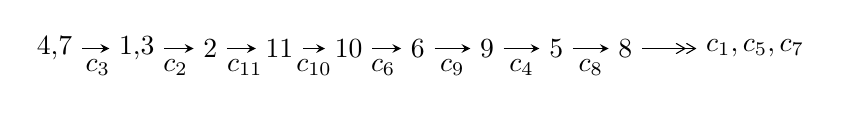
\begin{tikzpicture}[x=25pt, y=7pt]
	% node
	\node (A0) at (-1/8, 0) {4,7};
	\node (A1) at (17/16, 0) {1,3};
	\node (A2) at (17/8, 0) {2};
	\node (A3) at (25/8, 0) {11};
	\node (A4) at (33/8, 0) {10};
	\node (A5) at (41/8, 0) {6};
	\node (A6) at (49/8, 0) {9};
	\node (A7) at (57/8, 0) {5};
	\node (A8) at (65/8, 0) {8};
	\node (C1) at (1/2, -1) {$c_{3}$};
	\node (C2) at (13/8, -1) {$c_{2}$};
	\node (C3) at (21/8, -1) {$c_{11}$};
	\node (C4) at (29/8, -1) {$c_{10}$};
	\node (C5) at (37/8, -1) {$c_{6}$};
	\node (C6) at (45/8, -1) {$c_{9}$};
	\node (C7) at (53/8, -1) {$c_{4}$};
	\node (C8) at (61/8, -1) {$c_{8}$};
	\node (A9) at (10, 0) {$c_{1},c_{5},c_{7}$};

	% edge
	\draw[->,>=stealth]	
	(A0) edge (A1) (A1) edge (A2) (A2) edge (A3) (A3) edge (A4) (A4) edge (A5) (A5) edge (A6) (A6) edge (A7) (A7) edge (A8) ;
	\draw[->>,>={angle 60}]	
	(A8) edge (A9);
\end{tikzpicture} \\ 

\end{tabular} \\

\footnotetext{
The image of knot diagram is generated by the software ``\textbf{Draw programme}" developed by Andrew Bartholomew(\url{http://www.layer8.co.uk/maths/draw/index.htm\#Running-draw}), where we modified some parts for our purpose(\url{https://github.com/CATsTAILs/LinksPainter}).
}\phantom \\ \newline 
\centering \textbf{Ideals for irreducible components\footnotemark of $X_{\text{par}}$} 
 
\begin{align*}
I^u_{1}&=\langle 
6 u^{12}-31 u^{11}+\cdots+77 b+51,\;-16 u^{12}-20 u^{11}+\cdots+77 a+18,\\
\phantom{I^u_{1}}&\phantom{= \langle  }u^{13}+9 u^{11}+u^{10}+29 u^9+6 u^8+37 u^7+10 u^6+14 u^5+3 u^4+5 u^3-2 u^2+u-1\rangle \\
I^u_{2}&=\langle 
27350 u^{11}-10434 u^{10}+\cdots+116501 b+508418,\\
\phantom{I^u_{2}}&\phantom{= \langle  }-702574 u^{11}+701168 u^{10}+\cdots+2213519 a-5780311,\\
\phantom{I^u_{2}}&\phantom{= \langle  }u^{12}- u^{11}+8 u^{10}-7 u^9+26 u^8-13 u^7+53 u^6+7 u^5+80 u^4+38 u^3+72 u^2+24 u+19\rangle \\
I^u_{3}&=\langle 
u^7+4 u^5- u^4+6 u^3-2 u^2+b+3 u,\;u^7+5 u^5- u^4+10 u^3-3 u^2+a+7 u-2,\\
\phantom{I^u_{3}}&\phantom{= \langle  }u^8+5 u^6- u^5+10 u^4-3 u^3+8 u^2-2 u+1\rangle \\
\\
\end{align*}
\raggedright * 3 irreducible components of $\dim_{\mathbb{C}}=0$, with total 33 representations.\\
\footnotetext{All coefficients of polynomials are rational numbers. But the coefficients are sometimes approximated in decimal forms when there is not enough margin.}
\newpage
\renewcommand{\arraystretch}{1}
\centering \section*{I. $I^u_{1}= \langle 6 u^{12}-31 u^{11}+\cdots+77 b+51,\;-16 u^{12}-20 u^{11}+\cdots+77 a+18,\;u^{13}+9 u^{11}+\cdots+u-1 \rangle$}
\flushleft \textbf{(i) Arc colorings}\\
\begin{tabular}{m{7pt} m{180pt} m{7pt} m{180pt} }
\flushright $a_{4}=$&$\begin{pmatrix}1\\0\end{pmatrix}$ \\
\flushright $a_{7}=$&$\begin{pmatrix}0\\u\end{pmatrix}$ \\
\flushright $a_{1}=$&$\begin{pmatrix}0.207792 u^{12}+0.259740 u^{11}+\cdots+0.246753 u-0.233766\\-0.0779221 u^{12}+0.402597 u^{11}+\cdots+1.53247 u-0.662338\end{pmatrix}$ \\
\flushright $a_{3}=$&$\begin{pmatrix}1\\u^2\end{pmatrix}$ \\
\flushright $a_{2}=$&$\begin{pmatrix}0.259740 u^{12}+0.324675 u^{11}+\cdots-0.441558 u+1.20779\\-0.376623 u^{12}-0.220779 u^{11}+\cdots+0.740260 u+0.298701\end{pmatrix}$ \\
\flushright $a_{11}=$&$\begin{pmatrix}0.129870 u^{12}+0.662338 u^{11}+\cdots+1.77922 u-0.896104\\-0.0779221 u^{12}+0.402597 u^{11}+\cdots+1.53247 u-0.662338\end{pmatrix}$ \\
\flushright $a_{10}=$&$\begin{pmatrix}0.129870 u^{12}+0.662338 u^{11}+\cdots+1.77922 u-0.896104\\u\end{pmatrix}$ \\
\flushright $a_{6}=$&$\begin{pmatrix}-\frac{3}{7} u^{12}-\frac{2}{7} u^{11}+\cdots+\frac{10}{7} u-\frac{1}{7}\\-0.0779221 u^{12}+0.402597 u^{11}+\cdots+1.53247 u-0.662338\end{pmatrix}$ \\
\flushright $a_{9}=$&$\begin{pmatrix}0.129870 u^{12}+0.662338 u^{11}+\cdots+0.779221 u-0.896104\\u\end{pmatrix}$ \\
\flushright $a_{5}=$&$\begin{pmatrix}-0.662338 u^{12}-0.0779221 u^{11}+\cdots+1.02597 u+0.870130\\- u^2\end{pmatrix}$ \\
\flushright $a_{8}=$&$\begin{pmatrix}0.207792 u^{12}+0.259740 u^{11}+\cdots-0.753247 u-0.233766\\u^3+u\end{pmatrix}$\\ \flushright $a_{8}=$&$\begin{pmatrix}0.207792 u^{12}+0.259740 u^{11}+\cdots-0.753247 u-0.233766\\u^3+u\end{pmatrix}$\\&\end{tabular}
\flushleft \textbf{(ii) Obstruction class $= -1$}\\~\\
\flushleft \textbf{(iii) Cusp Shapes $= \frac{222}{77} u^{12}+\frac{8}{77} u^{11}+\frac{2008}{77} u^{10}+\frac{345}{77} u^9+\frac{6465}{77} u^8+26 u^7+\frac{8137}{77} u^6+\frac{3748}{77} u^5+\frac{2942}{77} u^4+\frac{285}{11} u^3+\frac{1313}{77} u^2-\frac{54}{77} u+\frac{501}{77}$}\\~\\
\newpage\renewcommand{\arraystretch}{1}
\flushleft \textbf{(iv) u-Polynomials at the component}\newline \\
\begin{tabular}{m{50pt}|m{274pt}}
Crossings & \hspace{64pt}u-Polynomials at each crossing \\
\hline $$\begin{aligned}c_{1},c_{5}\end{aligned}$$&$\begin{aligned}
&u^{13}-6 u^{12}+\cdots+26 u-4
\end{aligned}$\\
\hline $$\begin{aligned}c_{2}\end{aligned}$$&$\begin{aligned}
&u^{13}+8 u^{12}+\cdots+124 u-16
\end{aligned}$\\
\hline $$\begin{aligned}c_{3},c_{4},c_{8}\\c_{9}\end{aligned}$$&$\begin{aligned}
&u^{13}+9 u^{11}+\cdots+u-1
\end{aligned}$\\
\hline $$\begin{aligned}c_{6},c_{10}\end{aligned}$$&$\begin{aligned}
&u^{13}-9 u^{12}+\cdots+40 u-8
\end{aligned}$\\
\hline $$\begin{aligned}c_{7}\end{aligned}$$&$\begin{aligned}
&u^{13}-2 u^{12}+\cdots-7 u-1
\end{aligned}$\\
\hline $$\begin{aligned}c_{11}\end{aligned}$$&$\begin{aligned}
&u^{13}-2 u^{12}+\cdots-6 u-1
\end{aligned}$\\
\hline
\end{tabular}\\~\\
\newpage\renewcommand{\arraystretch}{1}
\flushleft \textbf{(v) Riley Polynomials at the component}\newline \\
\begin{tabular}{m{50pt}|m{274pt}}
Crossings & \hspace{64pt}Riley Polynomials at each crossing \\
\hline $$\begin{aligned}c_{1},c_{5}\end{aligned}$$&$\begin{aligned}
&y^{13}+8 y^{12}+\cdots+124 y-16
\end{aligned}$\\
\hline $$\begin{aligned}c_{2}\end{aligned}$$&$\begin{aligned}
&y^{13}-4 y^{12}+\cdots+31600 y-256
\end{aligned}$\\
\hline $$\begin{aligned}c_{3},c_{4},c_{8}\\c_{9}\end{aligned}$$&$\begin{aligned}
&y^{13}+18 y^{12}+\cdots-3 y-1
\end{aligned}$\\
\hline $$\begin{aligned}c_{6},c_{10}\end{aligned}$$&$\begin{aligned}
&y^{13}-3 y^{12}+\cdots+352 y-64
\end{aligned}$\\
\hline $$\begin{aligned}c_{7}\end{aligned}$$&$\begin{aligned}
&y^{13}+26 y^{12}+\cdots+53 y-1
\end{aligned}$\\
\hline $$\begin{aligned}c_{11}\end{aligned}$$&$\begin{aligned}
&y^{13}-24 y^{12}+\cdots+50 y-1
\end{aligned}$\\
\hline
\end{tabular}\\~\\
\newpage\flushleft \textbf{(vi) Complex Volumes and Cusp Shapes}
$$\begin{array}{c|c|c}  
\text{Solutions to }I^u_{1}& \I (\text{vol} + \sqrt{-1}CS) & \text{Cusp shape}\\
 \hline 
\begin{aligned}
u &= -0.589003 + 0.398981 I \\
a &= -0.155544 + 0.694999 I \\
b &= -0.701578 - 0.113111 I\end{aligned}
 & -1.89853 - 1.81856 I & \phantom{-}3.56685 + 4.77795 I \\ \hline\begin{aligned}
u &= -0.589003 - 0.398981 I \\
a &= -0.155544 - 0.694999 I \\
b &= -0.701578 + 0.113111 I\end{aligned}
 & -1.89853 + 1.81856 I & \phantom{-}3.56685 - 4.77795 I \\ \hline\begin{aligned}
u &= \phantom{-}0.313260 + 0.606523 I \\
a &= \phantom{-}0.71205 - 1.73803 I \\
b &= -0.241660 - 0.056194 I\end{aligned}
 & \phantom{-}1.23789 - 1.81241 I & \phantom{-}3.13803 - 1.59537 I \\ \hline\begin{aligned}
u &= \phantom{-}0.313260 - 0.606523 I \\
a &= \phantom{-}0.71205 + 1.73803 I \\
b &= -0.241660 + 0.056194 I\end{aligned}
 & \phantom{-}1.23789 + 1.81241 I & \phantom{-}3.13803 + 1.59537 I \\ \hline\begin{aligned}
u &= -0.067844 + 0.603023 I \\
a &= \phantom{-}0.009402 + 0.327160 I \\
b &= -0.281404 + 1.089340 I\end{aligned}
 & \phantom{-}1.10712 + 2.64289 I & \phantom{-}2.15723 - 4.40909 I \\ \hline\begin{aligned}
u &= -0.067844 - 0.603023 I \\
a &= \phantom{-}0.009402 - 0.327160 I \\
b &= -0.281404 - 1.089340 I\end{aligned}
 & \phantom{-}1.10712 - 2.64289 I & \phantom{-}2.15723 + 4.40909 I \\ \hline\begin{aligned}
u &= \phantom{-}0.435514\phantom{ +0.000000I} \\
a &= \phantom{-}0.789752\phantom{ +0.000000I} \\
b &= \phantom{-}0.240167\phantom{ +0.000000I}\end{aligned}
 & \phantom{-}0.684474\phantom{ +0.000000I} & \phantom{-}14.6290\phantom{ +0.000000I} \\ \hline\begin{aligned}
u &= -0.15240 + 1.67572 I \\
a &= \phantom{-}1.291360 - 0.096165 I \\
b &= -2.11530 - 0.55305 I\end{aligned}
 & -12.27390 - 4.64857 I & \phantom{-}3.70723 + 2.31166 I \\ \hline\begin{aligned}
u &= -0.15240 - 1.67572 I \\
a &= \phantom{-}1.291360 + 0.096165 I \\
b &= -2.11530 + 0.55305 I\end{aligned}
 & -12.27390 + 4.64857 I & \phantom{-}3.70723 - 2.31166 I \\ \hline\begin{aligned}
u &= -0.07312 + 1.68645 I \\
a &= -1.339690 - 0.391716 I \\
b &= \phantom{-}2.00168 - 0.40120 I\end{aligned}
 & -16.5929 - 2.0437 I & \phantom{-}1.74217 + 0.86236 I\\
 \hline 
 \end{array}$$\newpage$$\begin{array}{c|c|c}  
\text{Solutions to }I^u_{1}& \I (\text{vol} + \sqrt{-1}CS) & \text{Cusp shape}\\
 \hline 
\begin{aligned}
u &= -0.07312 - 1.68645 I \\
a &= -1.339690 + 0.391716 I \\
b &= \phantom{-}2.00168 + 0.40120 I\end{aligned}
 & -16.5929 + 2.0437 I & \phantom{-}1.74217 - 0.86236 I \\ \hline\begin{aligned}
u &= \phantom{-}0.35135 + 1.77586 I \\
a &= -1.41246 + 0.16455 I \\
b &= \phantom{-}2.21818 - 0.62507 I\end{aligned}
 & -17.1576 + 11.0164 I & \phantom{-}1.87407 - 4.91060 I \\ \hline\begin{aligned}
u &= \phantom{-}0.35135 - 1.77586 I \\
a &= -1.41246 - 0.16455 I \\
b &= \phantom{-}2.21818 + 0.62507 I\end{aligned}
 & -17.1576 - 11.0164 I & \phantom{-}1.87407 + 4.91060 I\\
 \hline 
 \end{array}$$\newpage\newpage\renewcommand{\arraystretch}{1}
\centering \section*{II. $I^u_{2}= \langle 27350 u^{11}-10434 u^{10}+\cdots+116501 b+508418,\;-7.03\times10^{5} u^{11}+7.01\times10^{5} u^{10}+\cdots+2.21\times10^{6} a-5.78\times10^{6},\;u^{12}- u^{11}+\cdots+24 u+19 \rangle$}
\flushleft \textbf{(i) Arc colorings}\\
\begin{tabular}{m{7pt} m{180pt} m{7pt} m{180pt} }
\flushright $a_{4}=$&$\begin{pmatrix}1\\0\end{pmatrix}$ \\
\flushright $a_{7}=$&$\begin{pmatrix}0\\u\end{pmatrix}$ \\
\flushright $a_{1}=$&$\begin{pmatrix}0.317401 u^{11}-0.316766 u^{10}+\cdots+11.2217 u+2.61137\\-0.234762 u^{11}+0.0895615 u^{10}+\cdots-7.84627 u-4.36407\end{pmatrix}$ \\
\flushright $a_{3}=$&$\begin{pmatrix}1\\u^2\end{pmatrix}$ \\
\flushright $a_{2}=$&$\begin{pmatrix}0.537344 u^{11}-0.633335 u^{10}+\cdots+18.5569 u+3.49184\\-0.413104 u^{11}+0.358821 u^{10}+\cdots-14.9788 u-5.59521\end{pmatrix}$ \\
\flushright $a_{11}=$&$\begin{pmatrix}0.0826395 u^{11}-0.227205 u^{10}+\cdots+3.37538 u-1.75270\\-0.234762 u^{11}+0.0895615 u^{10}+\cdots-7.84627 u-4.36407\end{pmatrix}$ \\
\flushright $a_{10}=$&$\begin{pmatrix}0.0826395 u^{11}-0.227205 u^{10}+\cdots+3.37538 u-1.75270\\-0.131415 u^{11}+0.0852353 u^{10}+\cdots-5.94685 u-1.61733\end{pmatrix}$ \\
\flushright $a_{6}=$&$\begin{pmatrix}0.0300079 u^{11}-0.174573 u^{10}+\cdots-0.414089 u-3.01586\\-0.0241200 u^{11}+0.170445 u^{10}+\cdots-0.572871 u+4.03170\end{pmatrix}$ \\
\flushright $a_{9}=$&$\begin{pmatrix}0.214055 u^{11}-0.312440 u^{10}+\cdots+9.32223 u-0.135373\\-0.131415 u^{11}+0.0852353 u^{10}+\cdots-5.94685 u-1.61733\end{pmatrix}$ \\
\flushright $a_{5}=$&$\begin{pmatrix}-0.118075 u^{11}-0.244437 u^{10}+\cdots-10.4369 u-12.7712\\-0.0941194 u^{11}+0.432511 u^{10}+\cdots+2.19875 u+7.10565\end{pmatrix}$ \\
\flushright $a_{8}=$&$\begin{pmatrix}-0.674354 u^{11}+0.991579 u^{10}+\cdots-19.6620 u+0.118551\\0.516880 u^{11}-0.642235 u^{10}+\cdots+16.6038 u+4.18226\end{pmatrix}$\\ \flushright $a_{8}=$&$\begin{pmatrix}-0.674354 u^{11}+0.991579 u^{10}+\cdots-19.6620 u+0.118551\\0.516880 u^{11}-0.642235 u^{10}+\cdots+16.6038 u+4.18226\end{pmatrix}$\\&\end{tabular}
\flushleft \textbf{(ii) Obstruction class $= -1$}\\~\\
\flushleft \textbf{(iii) Cusp Shapes $= -\frac{7968}{116501} u^{11}+\frac{34084}{116501} u^{10}+\cdots-\frac{122912}{116501} u-\frac{631486}{116501}$}\\~\\
\newpage\renewcommand{\arraystretch}{1}
\flushleft \textbf{(iv) u-Polynomials at the component}\newline \\
\begin{tabular}{m{50pt}|m{274pt}}
Crossings & \hspace{64pt}u-Polynomials at each crossing \\
\hline $$\begin{aligned}c_{1},c_{5}\end{aligned}$$&$\begin{aligned}
&(u^3+u^2+2 u+1)^4
\end{aligned}$\\
\hline $$\begin{aligned}c_{2}\end{aligned}$$&$\begin{aligned}
&(u^3+3 u^2+2 u-1)^4
\end{aligned}$\\
\hline $$\begin{aligned}c_{3},c_{4},c_{8}\\c_{9}\end{aligned}$$&$\begin{aligned}
&u^{12}- u^{11}+\cdots+24 u+19
\end{aligned}$\\
\hline $$\begin{aligned}c_{6},c_{10}\end{aligned}$$&$\begin{aligned}
&(u^2+u+1)^6
\end{aligned}$\\
\hline $$\begin{aligned}c_{7}\end{aligned}$$&$\begin{aligned}
&u^{12}+5 u^{11}+\cdots+96 u+37
\end{aligned}$\\
\hline $$\begin{aligned}c_{11}\end{aligned}$$&$\begin{aligned}
&u^{12}-3 u^{11}+\cdots+18 u+19
\end{aligned}$\\
\hline
\end{tabular}\\~\\
\newpage\renewcommand{\arraystretch}{1}
\flushleft \textbf{(v) Riley Polynomials at the component}\newline \\
\begin{tabular}{m{50pt}|m{274pt}}
Crossings & \hspace{64pt}Riley Polynomials at each crossing \\
\hline $$\begin{aligned}c_{1},c_{5}\end{aligned}$$&$\begin{aligned}
&(y^3+3 y^2+2 y-1)^4
\end{aligned}$\\
\hline $$\begin{aligned}c_{2}\end{aligned}$$&$\begin{aligned}
&(y^3-5 y^2+10 y-1)^4
\end{aligned}$\\
\hline $$\begin{aligned}c_{3},c_{4},c_{8}\\c_{9}\end{aligned}$$&$\begin{aligned}
&y^{12}+15 y^{11}+\cdots+2160 y+361
\end{aligned}$\\
\hline $$\begin{aligned}c_{6},c_{10}\end{aligned}$$&$\begin{aligned}
&(y^2+y+1)^6
\end{aligned}$\\
\hline $$\begin{aligned}c_{7}\end{aligned}$$&$\begin{aligned}
&y^{12}+19 y^{11}+\cdots-1224 y+1369
\end{aligned}$\\
\hline $$\begin{aligned}c_{11}\end{aligned}$$&$\begin{aligned}
&y^{12}-17 y^{11}+\cdots-2224 y+361
\end{aligned}$\\
\hline
\end{tabular}\\~\\
\newpage\flushleft \textbf{(vi) Complex Volumes and Cusp Shapes}
$$\begin{array}{c|c|c}  
\text{Solutions to }I^u_{2}& \I (\text{vol} + \sqrt{-1}CS) & \text{Cusp shape}\\
 \hline 
\begin{aligned}
u &= -0.538956 + 0.733343 I \\
a &= \phantom{-}0.564995 + 0.432837 I \\
b &= \phantom{-}0.527133 - 0.553665 I\end{aligned}
 & -3.82135 - 2.02988 I & \phantom{-}7.01951 + 3.46410 I \\ \hline\begin{aligned}
u &= -0.538956 - 0.733343 I \\
a &= \phantom{-}0.564995 - 0.432837 I \\
b &= \phantom{-}0.527133 + 0.553665 I\end{aligned}
 & -3.82135 + 2.02988 I & \phantom{-}7.01951 - 3.46410 I \\ \hline\begin{aligned}
u &= -0.230918 + 0.703145 I \\
a &= -0.20112 + 2.69084 I \\
b &= -0.69983 - 1.68387 I\end{aligned}
 & -7.95893 - 0.79824 I & \phantom{-}0.490245 - 0.484655 I \\ \hline\begin{aligned}
u &= -0.230918 - 0.703145 I \\
a &= -0.20112 - 2.69084 I \\
b &= -0.69983 + 1.68387 I\end{aligned}
 & -7.95893 + 0.79824 I & \phantom{-}0.490245 + 0.484655 I \\ \hline\begin{aligned}
u &= \phantom{-}0.161517 + 1.387090 I \\
a &= \phantom{-}1.002040 + 0.183839 I \\
b &= -1.65945 + 0.10008 I\end{aligned}
 & -3.82135 + 2.02988 I & \phantom{-}7.01951 - 3.46410 I \\ \hline\begin{aligned}
u &= \phantom{-}0.161517 - 1.387090 I \\
a &= \phantom{-}1.002040 - 0.183839 I \\
b &= -1.65945 - 0.10008 I\end{aligned}
 & -3.82135 - 2.02988 I & \phantom{-}7.01951 + 3.46410 I \\ \hline\begin{aligned}
u &= -0.22870 + 1.46755 I \\
a &= -1.84111 + 0.39110 I \\
b &= \phantom{-}2.46907 - 0.14826 I\end{aligned}
 & -7.95893 - 4.85801 I & \phantom{-}0.49024 + 6.44355 I \\ \hline\begin{aligned}
u &= -0.22870 - 1.46755 I \\
a &= -1.84111 - 0.39110 I \\
b &= \phantom{-}2.46907 + 0.14826 I\end{aligned}
 & -7.95893 + 4.85801 I & \phantom{-}0.49024 - 6.44355 I \\ \hline\begin{aligned}
u &= \phantom{-}1.31249 + 1.08009 I \\
a &= -0.043037 - 0.415642 I \\
b &= -0.507847 + 0.209151 I\end{aligned}
 & -7.95893 + 4.85801 I & \phantom{-}0.49024 - 6.44355 I \\ \hline\begin{aligned}
u &= \phantom{-}1.31249 - 1.08009 I \\
a &= -0.043037 + 0.415642 I \\
b &= -0.507847 - 0.209151 I\end{aligned}
 & -7.95893 - 4.85801 I & \phantom{-}0.49024 + 6.44355 I\\
 \hline 
 \end{array}$$\newpage$$\begin{array}{c|c|c}  
\text{Solutions to }I^u_{2}& \I (\text{vol} + \sqrt{-1}CS) & \text{Cusp shape}\\
 \hline 
\begin{aligned}
u &= \phantom{-}0.02457 + 1.83546 I \\
a &= -0.902821 + 0.085368 I \\
b &= \phantom{-}1.370920 + 0.193309 I\end{aligned}
 & -7.95893 + 0.79824 I & \phantom{-}0.490245 + 0.484655 I \\ \hline\begin{aligned}
u &= \phantom{-}0.02457 - 1.83546 I \\
a &= -0.902821 - 0.085368 I \\
b &= \phantom{-}1.370920 - 0.193309 I\end{aligned}
 & -7.95893 - 0.79824 I & \phantom{-}0.490245 - 0.484655 I\\
 \hline 
 \end{array}$$\newpage\newpage\renewcommand{\arraystretch}{1}
\centering \section*{III. $I^u_{3}= \langle u^7+4 u^5- u^4+6 u^3-2 u^2+b+3 u,\;u^7+5 u^5- u^4+10 u^3-3 u^2+a+7 u-2,\;u^8+5 u^6- u^5+10 u^4-3 u^3+8 u^2-2 u+1 \rangle$}
\flushleft \textbf{(i) Arc colorings}\\
\begin{tabular}{m{7pt} m{180pt} m{7pt} m{180pt} }
\flushright $a_{4}=$&$\begin{pmatrix}1\\0\end{pmatrix}$ \\
\flushright $a_{7}=$&$\begin{pmatrix}0\\u\end{pmatrix}$ \\
\flushright $a_{1}=$&$\begin{pmatrix}- u^7-5 u^5+u^4-10 u^3+3 u^2-7 u+2\\- u^7-4 u^5+u^4-6 u^3+2 u^2-3 u\end{pmatrix}$ \\
\flushright $a_{3}=$&$\begin{pmatrix}1\\u^2\end{pmatrix}$ \\
\flushright $a_{2}=$&$\begin{pmatrix}u^4+3 u^2+4\\- u^7-4 u^5+u^4-6 u^3+3 u^2-3 u+1\end{pmatrix}$ \\
\flushright $a_{11}=$&$\begin{pmatrix}-2 u^7-9 u^5+2 u^4-16 u^3+5 u^2-10 u+2\\- u^7-4 u^5+u^4-6 u^3+2 u^2-3 u\end{pmatrix}$ \\
\flushright $a_{10}=$&$\begin{pmatrix}-2 u^7-9 u^5+2 u^4-16 u^3+5 u^2-10 u+2\\- u\end{pmatrix}$ \\
\flushright $a_{6}=$&$\begin{pmatrix}u^7+u^6+6 u^5+3 u^4+12 u^3+2 u^2+9 u-1\\u^7+4 u^5- u^4+6 u^3-2 u^2+3 u\end{pmatrix}$ \\
\flushright $a_{9}=$&$\begin{pmatrix}-2 u^7-9 u^5+2 u^4-16 u^3+5 u^2-9 u+2\\- u\end{pmatrix}$ \\
\flushright $a_{5}=$&$\begin{pmatrix}u^6+4 u^4- u^3+7 u^2-2 u+3\\- u^2\end{pmatrix}$ \\
\flushright $a_{8}=$&$\begin{pmatrix}- u^7-5 u^5+u^4-9 u^3+3 u^2-6 u+2\\- u^3- u\end{pmatrix}$\\ \flushright $a_{8}=$&$\begin{pmatrix}- u^7-5 u^5+u^4-9 u^3+3 u^2-6 u+2\\- u^3- u\end{pmatrix}$\\&\end{tabular}
\flushleft \textbf{(ii) Obstruction class $= 1$}\\~\\
\flushleft \textbf{(iii) Cusp Shapes $= u^7+u^6+5 u^5+7 u^4+10 u^3+15 u^2+5 u+14$}\\~\\
\newpage\renewcommand{\arraystretch}{1}
\flushleft \textbf{(iv) u-Polynomials at the component}\newline \\
\begin{tabular}{m{50pt}|m{274pt}}
Crossings & \hspace{64pt}u-Polynomials at each crossing \\
\hline $$\begin{aligned}c_{1}\end{aligned}$$&$\begin{aligned}
&u^8- u^7+3 u^6-2 u^5+4 u^4-2 u^3+4 u^2- u+1
\end{aligned}$\\
\hline $$\begin{aligned}c_{2}\end{aligned}$$&$\begin{aligned}
&u^8+5 u^7+13 u^6+24 u^5+32 u^4+30 u^3+20 u^2+7 u+1
\end{aligned}$\\
\hline $$\begin{aligned}c_{3},c_{8},c_{9}\end{aligned}$$&$\begin{aligned}
&u^8+5 u^6- u^5+10 u^4-3 u^3+8 u^2-2 u+1
\end{aligned}$\\
\hline $$\begin{aligned}c_{4}\end{aligned}$$&$\begin{aligned}
&u^8+5 u^6+u^5+10 u^4+3 u^3+8 u^2+2 u+1
\end{aligned}$\\
\hline $$\begin{aligned}c_{5}\end{aligned}$$&$\begin{aligned}
&u^8+u^7+3 u^6+2 u^5+4 u^4+2 u^3+4 u^2+u+1
\end{aligned}$\\
\hline $$\begin{aligned}c_{6}\end{aligned}$$&$\begin{aligned}
&u^8-2 u^7+3 u^5-4 u^4+u^3+3 u^2-2 u+1
\end{aligned}$\\
\hline $$\begin{aligned}c_{7}\end{aligned}$$&$\begin{aligned}
&u^8-2 u^7+3 u^6+u^5-4 u^4+3 u^3-2 u+1
\end{aligned}$\\
\hline $$\begin{aligned}c_{10}\end{aligned}$$&$\begin{aligned}
&u^8+2 u^7-3 u^5-4 u^4- u^3+3 u^2+2 u+1
\end{aligned}$\\
\hline $$\begin{aligned}c_{11}\end{aligned}$$&$\begin{aligned}
&u^8-2 u^7+u^5+2 u^4-5 u^3+6 u^2-3 u+1
\end{aligned}$\\
\hline
\end{tabular}\\~\\
\newpage\renewcommand{\arraystretch}{1}
\flushleft \textbf{(v) Riley Polynomials at the component}\newline \\
\begin{tabular}{m{50pt}|m{274pt}}
Crossings & \hspace{64pt}Riley Polynomials at each crossing \\
\hline $$\begin{aligned}c_{1},c_{5}\end{aligned}$$&$\begin{aligned}
&y^8+5 y^7+13 y^6+24 y^5+32 y^4+30 y^3+20 y^2+7 y+1
\end{aligned}$\\
\hline $$\begin{aligned}c_{2}\end{aligned}$$&$\begin{aligned}
&y^8+y^7-7 y^6-4 y^5+36 y^4+70 y^3+44 y^2-9 y+1
\end{aligned}$\\
\hline $$\begin{aligned}c_{3},c_{4},c_{8}\\c_{9}\end{aligned}$$&$\begin{aligned}
&y^8+10 y^7+45 y^6+115 y^5+176 y^4+157 y^3+72 y^2+12 y+1
\end{aligned}$\\
\hline $$\begin{aligned}c_{6},c_{10}\end{aligned}$$&$\begin{aligned}
&y^8-4 y^7+4 y^6+y^5+4 y^4-13 y^3+5 y^2+2 y+1
\end{aligned}$\\
\hline $$\begin{aligned}c_{7}\end{aligned}$$&$\begin{aligned}
&y^8+2 y^7+5 y^6-13 y^5+4 y^4+y^3+4 y^2-4 y+1
\end{aligned}$\\
\hline $$\begin{aligned}c_{11}\end{aligned}$$&$\begin{aligned}
&y^8-4 y^7+8 y^6-9 y^5+4 y^4+5 y^3+10 y^2+3 y+1
\end{aligned}$\\
\hline
\end{tabular}\\~\\
\newpage\flushleft \textbf{(vi) Complex Volumes and Cusp Shapes}
$$\begin{array}{c|c|c}  
\text{Solutions to }I^u_{3}& \I (\text{vol} + \sqrt{-1}CS) & \text{Cusp shape}\\
 \hline 
\begin{aligned}
u &= \phantom{-}0.333178 + 1.212560 I \\
a &= \phantom{-}0.543877 + 0.445748 I \\
b &= -1.43305 - 0.31113 I\end{aligned}
 & -5.36621 + 1.77463 I & \phantom{-}0.03179 - 1.94850 I \\ \hline\begin{aligned}
u &= \phantom{-}0.333178 - 1.212560 I \\
a &= \phantom{-}0.543877 - 0.445748 I \\
b &= -1.43305 + 0.31113 I\end{aligned}
 & -5.36621 - 1.77463 I & \phantom{-}0.03179 + 1.94850 I \\ \hline\begin{aligned}
u &= \phantom{-}0.050347 + 1.305130 I \\
a &= \phantom{-}0.079860 + 0.540066 I \\
b &= -0.318291 + 0.506872 I\end{aligned}
 & -1.51415 + 3.01964 I & \phantom{-}3.37685 - 3.22289 I \\ \hline\begin{aligned}
u &= \phantom{-}0.050347 - 1.305130 I \\
a &= \phantom{-}0.079860 - 0.540066 I \\
b &= -0.318291 - 0.506872 I\end{aligned}
 & -1.51415 - 3.01964 I & \phantom{-}3.37685 + 3.22289 I \\ \hline\begin{aligned}
u &= -0.53500 + 1.45526 I \\
a &= -0.757549 + 0.849919 I \\
b &= \phantom{-}1.119420 - 0.799585 I\end{aligned}
 & -8.16060 - 3.11503 I & -0.52239 + 1.94780 I \\ \hline\begin{aligned}
u &= -0.53500 - 1.45526 I \\
a &= -0.757549 - 0.849919 I \\
b &= \phantom{-}1.119420 + 0.799585 I\end{aligned}
 & -8.16060 + 3.11503 I & -0.52239 - 1.94780 I \\ \hline\begin{aligned}
u &= \phantom{-}0.151478 + 0.362294 I \\
a &= \phantom{-}1.13381 - 1.98717 I \\
b &= -0.368086 - 0.741932 I\end{aligned}
 & \phantom{-}1.88148 - 2.34966 I & \phantom{-}12.61375 + 3.05058 I \\ \hline\begin{aligned}
u &= \phantom{-}0.151478 - 0.362294 I \\
a &= \phantom{-}1.13381 + 1.98717 I \\
b &= -0.368086 + 0.741932 I\end{aligned}
 & \phantom{-}1.88148 + 2.34966 I & \phantom{-}12.61375 - 3.05058 I\\
 \hline 
 \end{array}$$\newpage
\newpage\renewcommand{\arraystretch}{1}
\centering \section*{ IV. u-Polynomials}
\begin{tabular}{m{50pt}|m{274pt}}
Crossings & \hspace{64pt}u-Polynomials at each crossing \\
\hline $$\begin{aligned}c_{1}\end{aligned}$$&$\begin{aligned}
&(u^3+u^2+2 u+1)^4(u^8- u^7+3 u^6-2 u^5+4 u^4-2 u^3+4 u^2- u+1)\\
&\cdot(u^{13}-6 u^{12}+\cdots+26 u-4)
\end{aligned}$\\
\hline $$\begin{aligned}c_{2}\end{aligned}$$&$\begin{aligned}
&(u^3+3 u^2+2 u-1)^4\\
&\cdot(u^8+5 u^7+13 u^6+24 u^5+32 u^4+30 u^3+20 u^2+7 u+1)\\
&\cdot(u^{13}+8 u^{12}+\cdots+124 u-16)
\end{aligned}$\\
\hline $$\begin{aligned}c_{3},c_{8},c_{9}\end{aligned}$$&$\begin{aligned}
&(u^8+5 u^6+\cdots-2 u+1)(u^{12}- u^{11}+\cdots+24 u+19)\\
&\cdot(u^{13}+9 u^{11}+\cdots+u-1)
\end{aligned}$\\
\hline $$\begin{aligned}c_{4}\end{aligned}$$&$\begin{aligned}
&(u^8+5 u^6+\cdots+2 u+1)(u^{12}- u^{11}+\cdots+24 u+19)\\
&\cdot(u^{13}+9 u^{11}+\cdots+u-1)
\end{aligned}$\\
\hline $$\begin{aligned}c_{5}\end{aligned}$$&$\begin{aligned}
&(u^3+u^2+2 u+1)^4(u^8+u^7+3 u^6+2 u^5+4 u^4+2 u^3+4 u^2+u+1)\\
&\cdot(u^{13}-6 u^{12}+\cdots+26 u-4)
\end{aligned}$\\
\hline $$\begin{aligned}c_{6}\end{aligned}$$&$\begin{aligned}
&(u^2+u+1)^6(u^8-2 u^7+3 u^5-4 u^4+u^3+3 u^2-2 u+1)\\
&\cdot(u^{13}-9 u^{12}+\cdots+40 u-8)
\end{aligned}$\\
\hline $$\begin{aligned}c_{7}\end{aligned}$$&$\begin{aligned}
&(u^8-2 u^7+\cdots-2 u+1)(u^{12}+5 u^{11}+\cdots+96 u+37)\\
&\cdot(u^{13}-2 u^{12}+\cdots-7 u-1)
\end{aligned}$\\
\hline $$\begin{aligned}c_{10}\end{aligned}$$&$\begin{aligned}
&(u^2+u+1)^6(u^8+2 u^7-3 u^5-4 u^4- u^3+3 u^2+2 u+1)\\
&\cdot(u^{13}-9 u^{12}+\cdots+40 u-8)
\end{aligned}$\\
\hline $$\begin{aligned}c_{11}\end{aligned}$$&$\begin{aligned}
&(u^8-2 u^7+\cdots-3 u+1)(u^{12}-3 u^{11}+\cdots+18 u+19)\\
&\cdot(u^{13}-2 u^{12}+\cdots-6 u-1)
\end{aligned}$\\
\hline
\end{tabular}\newpage\renewcommand{\arraystretch}{1}
\centering \section*{ V. Riley Polynomials}
\begin{tabular}{m{50pt}|m{274pt}}
Crossings & \hspace{64pt}Riley Polynomials at each crossing \\
\hline $$\begin{aligned}c_{1},c_{5}\end{aligned}$$&$\begin{aligned}
&(y^3+3 y^2+2 y-1)^4\\
&\cdot(y^8+5 y^7+13 y^6+24 y^5+32 y^4+30 y^3+20 y^2+7 y+1)\\
&\cdot(y^{13}+8 y^{12}+\cdots+124 y-16)
\end{aligned}$\\
\hline $$\begin{aligned}c_{2}\end{aligned}$$&$\begin{aligned}
&(y^3-5 y^2+10 y-1)^4\\
&\cdot(y^8+y^7-7 y^6-4 y^5+36 y^4+70 y^3+44 y^2-9 y+1)\\
&\cdot(y^{13}-4 y^{12}+\cdots+31600 y-256)
\end{aligned}$\\
\hline $$\begin{aligned}c_{3},c_{4},c_{8}\\c_{9}\end{aligned}$$&$\begin{aligned}
&(y^8+10 y^7+45 y^6+115 y^5+176 y^4+157 y^3+72 y^2+12 y+1)\\
&\cdot(y^{12}+15 y^{11}+\cdots+2160 y+361)(y^{13}+18 y^{12}+\cdots-3 y-1)
\end{aligned}$\\
\hline $$\begin{aligned}c_{6},c_{10}\end{aligned}$$&$\begin{aligned}
&(y^2+y+1)^6(y^8-4 y^7+4 y^6+y^5+4 y^4-13 y^3+5 y^2+2 y+1)\\
&\cdot(y^{13}-3 y^{12}+\cdots+352 y-64)
\end{aligned}$\\
\hline $$\begin{aligned}c_{7}\end{aligned}$$&$\begin{aligned}
&(y^8+2 y^7+5 y^6-13 y^5+4 y^4+y^3+4 y^2-4 y+1)\\
&\cdot(y^{12}+19 y^{11}+\cdots-1224 y+1369)(y^{13}+26 y^{12}+\cdots+53 y-1)
\end{aligned}$\\
\hline $$\begin{aligned}c_{11}\end{aligned}$$&$\begin{aligned}
&(y^8-4 y^7+8 y^6-9 y^5+4 y^4+5 y^3+10 y^2+3 y+1)\\
&\cdot(y^{12}-17 y^{11}+\cdots-2224 y+361)(y^{13}-24 y^{12}+\cdots+50 y-1)
\end{aligned}$\\
\hline
\end{tabular}
\vskip 2pc
\end{document}